\chapter{Reference Model}
\label{ch:Reference Model}

The main challenges discussed in \cref{sec:back_issProblem} are that when using an ISS as a reference model, asynchronous events can be taken at the wrong time, and the timing of the side effects can vary between the DUT and the reference model.
This chapter will discuss multiple design choices to build a Reference Model that solves these challenges. To overcome these challenges, we should add a pipeline understanding to the model and use this to time asynchronous events and side effects correctly.

Additionally, the model should be easily adaptable to different processor cores with different amounts of pipeline stages, allow for custom instructions to be easily integrated, and be easy to maintain. To achieve this, we will evaluate various design options in the following sections to find an optimal solution to meet the requirements. In \cref{sec:architecture}, we will discuss the basic architecture of the model, partitioning the design into a pipeline shell and an ISS. \Cref{sec:inOut} will cover the inputs and outputs to the model, \cref{sec:shell_iss_interaction} will discuss the different options for the interaction and partitioning of the model into the pipeline shell and the ISS. \Cref{sec:pipelineShell} will cover the implementation choices for the pipeline shell, and \cref{sec:choosingISS} will compare different Instruction Set Simulators to use in the reference model.


%\section{Reference model design}
%
%\subsection{Design choices}
%
%\begin{itemize}
%    \item Basic architecture
%    \item Instruction inputs to the model. ELF vs UVM monitor vs RVFI input
%    \item Asynchronous inputs to the model. UVM monitor vs RVFI vs RVVI
%    \item Outputs from the model. RVFI
%    \item Communication between ISS and Pipeline Shell. Closely linked vs Pipeline shell then ISS vs ISS then Pipeline shell.
%    \item Pipeline shell implementation. Full simulation vs. ImperasDV vs. Simplified simulation
%    \item Which ISS to build around
%    \item Core configuration. How can the model account for different cores. What parts could be shared and which are core dependent.
%\end{itemize}

\section{Reference Model Architecture}
\label{sec:architecture}

The architecture of the Reference Model can be designed in various ways. This section will cover modeling the simulator using a micro-architectural simulator or an Instruction Set Simulator (ISS).

\subsection{Model based on a Micro-architectural simulator}

One approach is to build a reference model that architecturally operates the same way as the processor. This can be done either by modifying an existing micro-architectural simulator such as Gem5 from \cref{sec:gem5} or MARSS-RISCV from \cref{sec:marss}, or building it from the ground up. Using or building a micro-architectural model would allow a highly specialized model to be modeled to the specific processor. This would be very accurate but has some disadvantages.

Building the entire simulator from the ground up around a specific core would be very time-consuming. A lot of the implementation would be to model core-independent RISC-V functionality, which already exists in ISSs. Additionally, building the system from the ground up increases the risk of introducing bugs into the model. Instead, we can use an existing micro-architectural simulator. These would then have to be modified both to support verification, like implementing lock-step execution and tracing, and the micro-architectural components need to be modified to support the verified core. These modifications also increase the risk of bugs. 

Both of these solutions also limit the reuse of components for different processor cores and would require invasive modifications to support different processor cores. Because the functionality is embedded into multiple micro-architectural components, the modifications for different cores can also modify the functionality and RISC-V compliance of the model.

One micro-architectural simulator we could use is MARSS-RISCV (\cref{sec:marss}). This is no longer in active development, with the last update in 2020. This is not ideal, as it would have to get the model back to an up-to-date state, and we could not rely on others to maintain the functionality and add new extensions.

Gem5 is another micro-architectural simulator, introduced in \cref{sec:gem5}.
It is powerful for architectural exploration and performance estimation but lacks some features useful in verification, like lock-step execution and trace output. The ability to insert custom instructions is also complicated. Gem5 already implements an in-order pipeline with its own intricacies. Since it already has a pipeline, modifying it to match the DUT core while ensuring the functionality is kept intact could be complicated. Gem5 also simulates close to the RTL level, meaning architectural bugs could be modeled in the DUT and Gem5 and not be found. \cite{noauthor_gem5_2023}


\subsection{Model based on an Instruction Set Simulator}

Another approach would be to utilize an existing ISS in the reference model. This can be done using a similar approach to the cycle-accurate simulators described in \Cref{sec:cycle-accurate}. One solution is a two-layered approach with one functional kernel and one timing shell. This partitioning allows the functional kernel to be independent of core specifics and be responsible for the functionality described in the ISA specification, while the timing shell is responsible for handling the core-specific timing of the pipeline and interaction with the rest of the system. This enhances the model's modularity, allowing the functional kernel to be reused for multiple cores, and only the timing shell requires modifications to fit different cores \cite{chiang_efficient_2009}.

Using this approach, we can use a partitioning where an existing ISS can be used as the functional kernel, and we can build a specialized timing shell on top, referred to as the \textit{pipeline shell}.
This can give the following advantages:

\begin{itemize}
    \item By using a widely tested and bug-free ISS, there are fewer possibilities of introducing bugs to the reference model. 
    \item The ISS can be kept updated and maintained to remove bugs, keep up to date with extensions, and support adding custom extensions.
    \item The ISS can be reused for multiple cores
\end{itemize}

However, a disadvantage is that we have to conform to the interface provided by the ISS or modify the ISS to fit the requirements needed in the model.

\subsection{Architecture}

Of the two approaches introduced above, the two-layered approach using an ISS achieves the best modularity, the lowest possibility of bugs, and is the easiest approach to ensure that the model is up-to-date in the future. Therefore, this approach will be used further to discuss the rest of the design choices in this chapter.

\Cref{fig:env-block-diagram} shows a basic block diagram of the verification environment and the organization of the Reference Model with the proposed partitioning of the Reference Model into a \textit{Pipeline Shell} and an existing Instruction Set Simulator. 

\begin{figure}[ht]
    \centering
    \includegraphics[width=0.75\linewidth]{pictures/ReferenceModelEnvironment.pdf}
    \caption{A simplified block diagram of the verification environment and Reference Model Architecture.}
    \label{fig:env-block-diagram}
\end{figure}

\section{Inputs and outputs to the reference model}
\label{sec:inOut}

This section will discuss the different choices of inputs and outputs from the reference model. The inputs to the model are instructions to execute, asynchronous interrupts, and asynchronous debug requests. To be used in a step-and-compare verification environment, the reference model should output the model's state changes through the RVFI interface described in \cref{sec:rvfi}. 

\subsection{Instruction inputs}

When loading instructions into the model, there are three choices: 
we can either load an entire ELF file into the reference model, 
use the instruction embedded in the RVFI item from the DUT, 
or use a UVM monitor to monitor the instruction being fetched from the instruction memory from the DUT.

Using the RVFI instructions and the instructions from the UVM monitor, the fetched instructions would follow the DUT. If the DUT fetches the wrong instruction, the reference model will also fetch the wrong instruction, and the bug will not be reported. If we load the ELF file into the reference model and separately fetch instructions from this file, we can verify if the DUT's instruction fetching works as intended. 

\subsection{Asynchronous inputs}

\subsubsection{RVFI triggered interrupt}

In the approach used in the step-and-compare 2.0 methodology explained in \cref{sec:core-v-verif}, the reference model is not to be directly connected to the interrupt and debug generator. Instead, asynchronous events are signaled to the reference model (RM) through the RVFI interface output from the DUT \cite{taylor_advanced_2023}.

When an asynchronous interrupt occurs in the DUT, it is notified over RVFI in the first retired instruction of the trap handler. To ensure the DUT and RM stay in sync, the RM will jump to the interrupt handler when the DUT reports the first instruction of the interrupt handler with \lstinline{rvfi_intr}.  If this is done, the DUT and RM will keep in sync as the RM is following the DUT.

However, this is somewhat problematic as we can not verify if the interrupt was taken at the correct time or if the correct interrupt was taken. Therefore, we need another method to verify if the correct interrupt was taken at the correct time \cite{taylor_advanced_2023}.
We also do not know when the asynchronous event happen, making the more advanced interrupt handling of the reference model difficult. 

\subsubsection{Interrupts triggered independently of RVFI}

To properly verify interrupts, we want to notify the reference model of interrupts independently of an RVFI instruction retirement when it arrives. 

As the core-v-verif environment currently uses RVVI to communicate with the reference model, as explained in \cref{sec:core-v-verif}, using RVVI to interface with our reference model is convenient, to allow the reference model to be replaced easier, without modifying the verification environment too much.

The RVVI-API supports this by setting the interrupt pin using the \lstinline{rvviRefNetSet(netIndex, value, when)} API. By using the \lstinline{when} parameter, we can specify which cycle the interrupt pins were set.

This approach allows us to see exactly at what clock cycle the interrupt appears, which allows us to properly simulate the correct timing of the interrupt.

%One possibility could be to look at the previous states when an interrupt happens and determine if an interrupt was allowed to happen. 
%
%We could possible "rebuild" the pipeline from the previous retired instructions, but not need to simulate the pipeline the entire time. 
%
%If the interrupt is inserted into the reference model at the right time, as well as being reported over rvfi....
%we could 



%\subsection{Types of reference models}
%
%cycle-accurate
%
%Discrete-event with time accounting models
%
%event models




%\subsection{Reference model parallel to core.}
%
%\begin{itemize}
%    \item Input is the same as the core input
%    \item Possibly use an uvm agent to listen to bus transactions and feed into reference model 
%    \item RVFI output
%    \item Pass/Fail done by comparing RFVI from core and reference model
%\end{itemize}

%\subsection{RVFI input}
%
%\begin{itemize}
%    \item Under normal execution, the pipeline is not simulated and the retired instruction from the core is fed into the ISS.
%    \item When the reference model gets notified about an interrupt, it must "backtrack" and calculate the pipeline state and corresponding side-effects.
%\end{itemize}


%To avoid the complications with simulating the entire pipeline, we might get away with only knowing what state changes happen in each state for each instruction.
%eg. what happens 2 cycles before instructions retire.


\section{Pipeline shell implementation}
\label{sec:pipelineShell}

The \textit{Pipeline shell} should be built on top of the ISS, simulating the timing of instructions through the pipeline, while the ISS simulates the functional execution of each instruction. This section will cover different approaches to modeling the pipeline shell.



\subsection{Full pipeline simulation}
\label{sec:fullPipeline}

The most accurate and complex simulation strategy is to simulate all the components of the pipeline, simulating all transitions, dependencies, stalls, etc, the same way the processor operates. This requires a tight coupling between the pipeline shell and the ISS, and it is necessary to split up the ISS into separate fetch, decode, execute, and writeback modules that are called from each corresponding stage from the pipeline shell. We also need to simulate all the intricacies of the pipeline, like hazards, forwarding, stalls, multi-cycle instructions, memory access, etc. 

This approach achieves very accurate results and fine-grained control over the behavior of the pipeline. However, this approach is challenging to implement and is very specialized to specific cores. Additionally, there is a risk of encountering the same bugs as the RTL implementation.

%
%We will detail what needs to be simulated for each pipeline stage below, using the CV32E40X as an example.
%
%\subsubsection{IF}
%The IF stage should simulate fetching the next instruction from memory. It should simulate memory access timing, pipeline stalls from cache misses, memory latency, etc. 
%
%
%\subsubsection{ID}
%
%To properly simulate the pipeline execution, we should simulate forwarding, dependencies, and hazards between instructions. Therefore, It is necessary to decode the instructions in this stage to extract the instruction type, registers, control signals, etc., necessary to calculate hazards. We should also read the values from the register file here to be used in the EX stage. In CV32E40X, jumps are taken from the ID stage and must also be simulated \cite{openhw_group_pipeline_2023}.
%
%\subsubsection{EX}
%
%In the EX stage, we must simulate all execution of instructions, including ALU, multiplication, and division. In the CV32E40X core, some instructions require multiple clock cycles to complete, so correct simulation of the EX stage requires stalling the EX stage for the correct number of clock cycles corresponding to the instruction type. Most instructions have a set number of clock cycles, while others have a variable amount. For instance, division and remainder operations can take between 3 and 35 cycles, depending on the operand value. This can be quite complicated and requires the simulator to simulate the division operation the same way as the core to get the correct amount of clock cycles. Alternatively, a simplified algorithm can be developed to determine the exact amount of clock cycles for a given operand.
%
%In addition, branches are taken from the EX stage, requiring calculation of the branch condition here. It must then take the branch, requiring a flush of IF and ID and a 3-4 cycle stall, or it must not take it.
%Additionally, the Load-Store-Unit (LSU) address generation and data requests are done in the EX stage.\cite{openhw_group_pipeline_2023}
%
%\subsubsection{WB}
%
%In the WB stage, the results are written to the correct registers. The second part of the LSU is also executed in the WB stage, so possible stalls from the LSU must be handled.
%
%In most Instruction Set Simulators (ISSs), the execution and write-back stages are combined into a single function. However, this approach can cause issues when using the execute function from the pipeline shell. The problem is that any changes made to the registers during this stage are immediately written back. As a result, it can lead to an inaccurate simulation if there are interruptions to program flow while in the EX stage that are finished in the ISS but then aborted in the actual implementation.\cite{openhw_group_pipeline_2023}
%
%We must modify the ISS to separate the execute and writeback functionality to solve this. This can be quite complicated as it changes fundamental parts of the operation of the ISS, and great care must be taken to ensure the ISS still operates correctly. Another solution could be to run the execute function in the writeback stage instead of the execute state. With this method, the effects of the instructions are correctly written back at the correct time. The disadvantage of this approach is that side effects from the execution will not be executed in the EX stage but in the WB stage. This could be solved with additional logic in the EX stage to execute these side effects in the EX stage.
%
%\subsubsection{Pipeline control}
%
%To properly model the pipeline, we need a module to determine when an instruction can advance to the next stage, considering stalls, multi-cycle operations, forwarding, data hazards, branch mispredictions, pipeline flushes, etc.
%
%
%\subsubsection{Interrupts}
%
%In this approach, the goal of accurately simulating the entire pipeline is for interrupts to be passed directly into the model at the correct time and for the model to simulate the handling correctly. 
%To determine when an interrupt can be taken, the model must check the contents of the pipeline stages and determine if all necessary conditions for an input to be taken are fulfilled. 
%If the interrupt can not be taken, it must halt the ID stage and continue executing instructions until all conditions apply.
%When the interrupt can be taken, it must flush the pipeline and load the interrupt handler correctly. \cite{openhw_group_exceptions_2023}

\subsection{Simplified Simulation} 


%In the following approach, we attempt to simplify the approach in \cref{sec:fullPipeline} by simulating only the essential components for correct verification of asynchronous events while abstracting away the rest.

To avoid unnecessary complexity, we only want to simulate the components necessary to verify asynchronous events properly while abstracting away the rest. Therefore, we propose the method below to find the optimal abstraction level of the pipeline shell.

\subsubsection{Finding the appropriate abstraction level}

\begin{enumerate}
    \item Find all requirements that affect the timing of interrupts.
    \item Analyze each requirement to identify the underlying requirements. 
    \item When all fundamental requirements are found, identify the necessary simulations to achieve each fundamental requirement, creating a dependency tree.
    \item Analyze the dependency tree to determine which abstractions can be done and which dependencies require accurate simulation.
\end{enumerate}

%\subsubsection{Simulation components}
%
%Components necessary to fully simulate the CV32E40X
%
%\begin{enumerate}
%    \item IF stage - Fetches 1 instruction per cycle, through an aligning prefetch buffer, if the memory allows.
%    \begin{itemize}
%        \item normal fetch
%        \item Bus error
%        \item Multiple outstanding memory transactions
%        \item Memory access delay
%        \item Misaligned accesses
%        \item stall - if instruction issued during single step
%    \end{itemize}
%    \item ID stage
%    \begin{itemize}
%        \item Instruction decoding
%        \item stalling - e.g. if pending interrupt 
%        \item Hazard if an instruction causing implicit CSR read in ID while csr access in WB
%        \item 2 cycle stall hazard if an instruction causing implicit CSR read in ID while csr access in WB
%        \item Jump happens from ID
%    \end{itemize}
%    \item EX stage
%    \begin{itemize}
%        \item Instruction execution
%        \item ALU, Multiplier, and Divider
%        \item Branches happen from EX if conditions are met
%        \item Stalls until multi-cycle instructions are complete. Multi-cycle instructions can be fixed or variable in length.
%        \item Address generation for Load-store-unit (LSU) is done in EX 
%    \end{itemize}
%    \item WB stage
%    \begin{itemize}
%        \item Write results back to register file
%        \item Second part of LSU. Takes one bus transaction for aligned and 2 misaligned transfers.
%        \item Simulate memory access delay 
%    \end{itemize}
%    \item Hazards
%    \item Stalls
%    \item Forwarding
%    \item Pipeline flushing
%    \item Branching
%    \item Jumps
%    \item CSR 
%    \item compressed instructions
%\end{enumerate}


To build a dependency tree for the CV32E40X core, we base the exploration on the RTL code in \cite{noauthor_openhw_2023}. From \lstinline{cv32e40x_controller_fsm.sv}, we can see that interrupts are taken if there is a pending interrupt and interrupt is allowed. Whether interrupts are allowed to be taken in CV32E40X depends on the following factors taken from the code:

\pagebreak

\begin{lstlisting}
  // Allow interrupts to be taken only if there is no data request in WB,
  // and no trans_valid has been clocked from EX to environment.
  // Not allowing interrupts when the core cannot take interrupts due to debug conditions.
  // Offloaded instructions in WB also block, as they cannot be killed after commit_kill=0 (EX stage)
  // LSU instructions which were suppressed due to previous exceptions or trigger match
  // will be interruptable as they were converted to NOP in ID stage.
  // When a fencei is present in WB and the LSU has completed all tranfers, the fencei handshake will be initiated. This must complete and the fencei instruction must retire before allowing interrupts.
  // Any multi operation instruction (table jumps, push/pop and double moves) may not be interrupted once the first operation has completed its operation in WB.
  //   - This is guarded with using the sequence_interruptible, which tracks sequence progress through the WB stage.
  // When a CLIC pointer is in the pipeline stages EX or WB, we must block interrupts.
  //   - Interrupt would otherwise kill the pointer and use the address of the pointer for mepc. A following mret would then return to the mtvt table, losing program progress. 
\end{lstlisting}

\begin{figure}[ht]
    \centering
    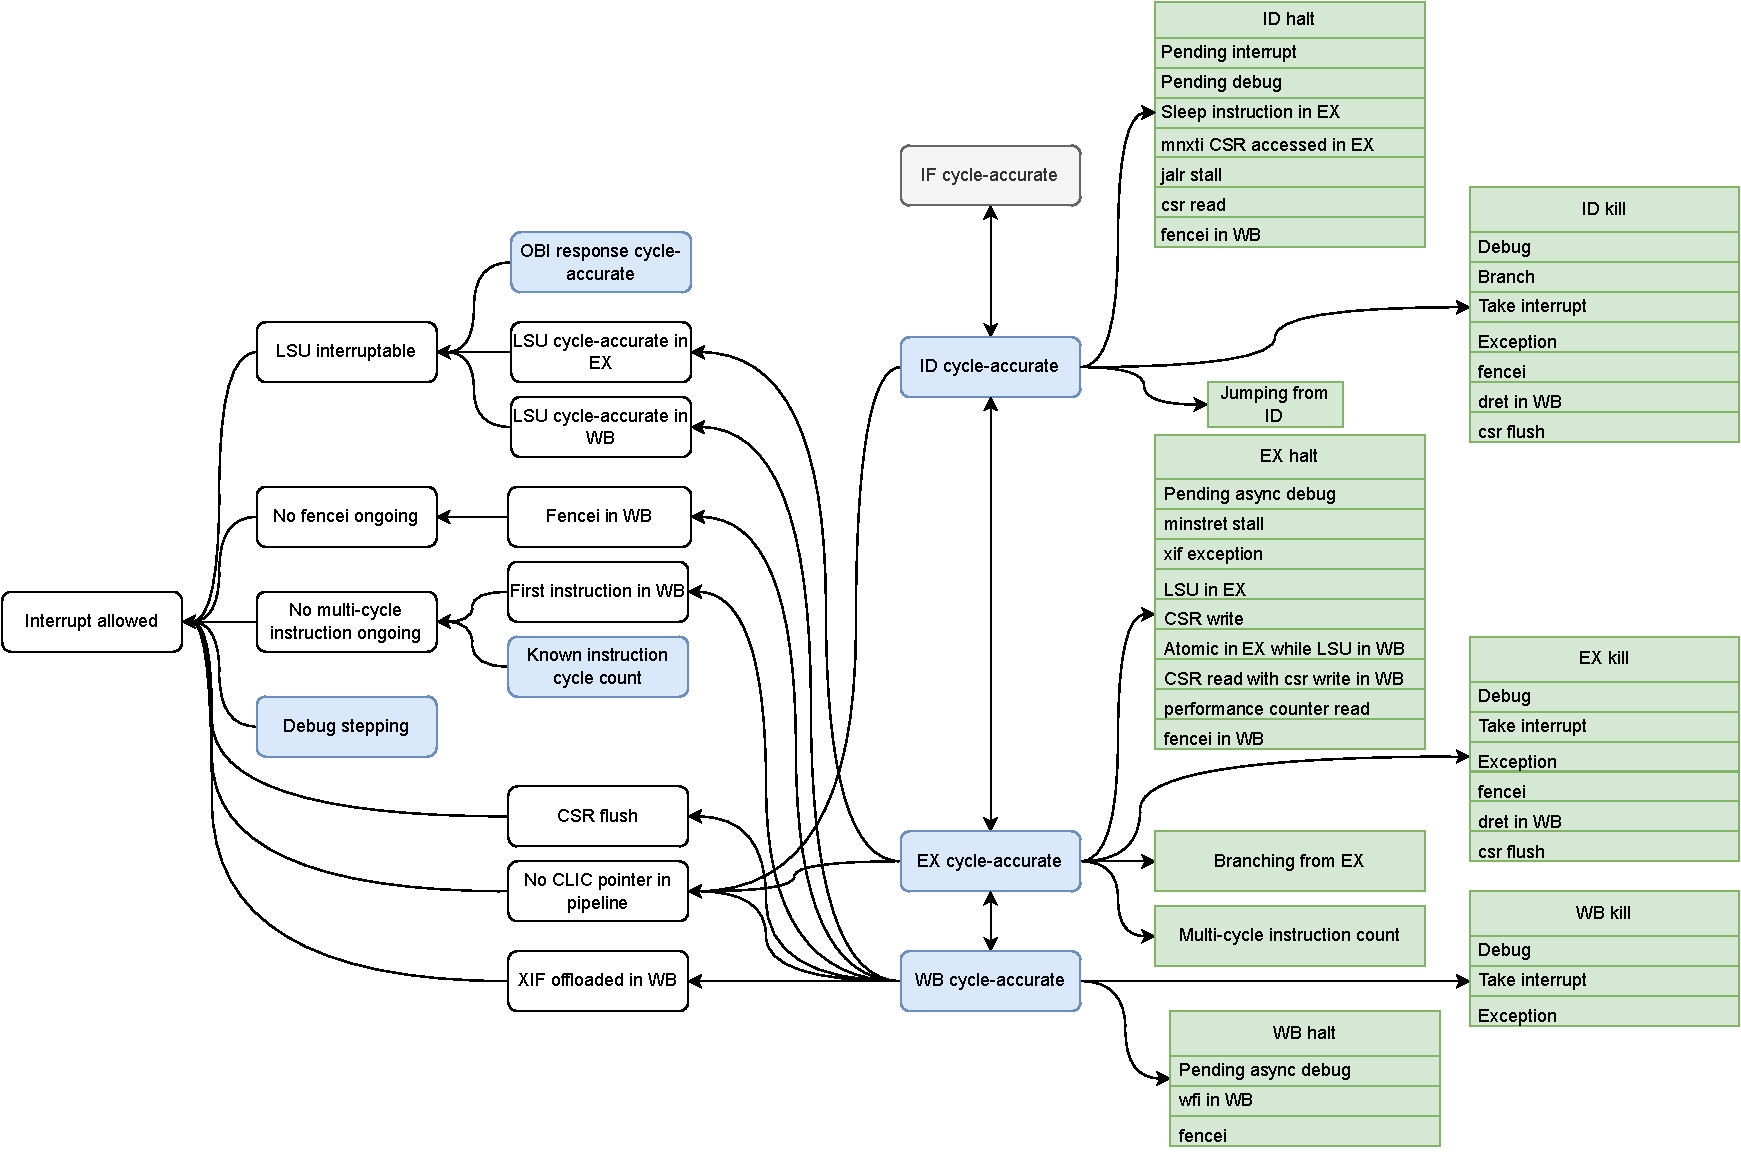
\includegraphics[width=1\linewidth]{pictures/Dependencies.pdf}
    \caption{Simulation dependency tree for interrupt handling in the CV32E40X core.}
    \label{fig:dependencyTree}
\end{figure}


We use this as a basis for building a dependency tree. The dependency tree is shown in \cref{fig:dependencyTree}. In the first layer, we see the following requirements:


\begin{itemize}
    \item The LSU is interruptable:
    %\begin{itemize}
    %    \item No data request in WB
    %    \item \lstinline{trans_valid} has not been clocked from EX
    %    \item The address phase is done, without finishing with \lstinline{resp_valid=1} in WB
    %    \item For misaligned split instructions, we may interrupt during the first cycle of the first half. If the first half stays in EX for more than one cycle, we cannot interrupt it (\lstinline{trans_valid_q == 1}). When the first half goes to WB, \lstinline{cnt_q != 0} will block interrupts. If the first half finishes in WB before the second half gets grant, \lstinline{trans_valid_q} will again be 1 and block interrupts, and \lstinline{cnt_q} will block the last half while it is in WB.
    %\end{itemize}
    \item When a fencei instruction is present in WB and the LSU has completed all tranfers, the fencei handshake will be initiated. This must complete and the fencei instruction must retire before allowing interrupts. 
    \item Don't allow interrupts in debug mode or single stepping without \lstinline{dcsr.stepie} set.
    \item Any multi-operation instruction may not be interrupted once the first operation has completed its operation in WB.
    \item Don't allow interrupts when a CLIC pointer is in the pipeline.
    \item Don't allow interrupts when a CSR flush happens
    \item Don't allow interrupts when an XIF instruction is offloaded in the WB.
    
\end{itemize}

From this, we can figure out what requirements are necessary. For the LSU to be interruptible, LSU instructions must be accurate in the EX and WB stage. We also need to know at which cycle the LSU gets a response via the OBI interface.
To know if a fencei transaction is in progress, we must know if the fencei instruction is in WB. To properly simulate multi-cycle instructions, we need to know when the first cycle has started by knowing if the first cycle is in WB, and we must know how many cycles the instruction will take. We must also know if we are in the debug mode, if there is a CLIC pointer in the pipeline, and if there is an offloaded XIF instruction in WB.

From these discoveries, we can deduce the fundamental requirements listed below, shown in blue in \cref{fig:dependencyTree}.
\begin{itemize}
    \item OBI response cycle-accurate
    \item Known instruction cycle count for multi-cycle instructions
    \item Debug stepping mode
    \item Instructions are cycle-accurate in the ID stage
    \item Instructions are cycle-accurate in the EX stage
    \item Instructions are cycle-accurate in the WB stage
\end{itemize}

From these requirements, we can determine what simulation components are necessary to accurately simulate the requirements above. These components are shown in green in \cref{fig:dependencyTree}. This shows that for each pipeline stage, we need to simulate halting and flushing of the stage, with all the requirements for halting and flushing shown in green. In addition, we must simulate jumping from the ID stage, branching from the EX stage, and accurate multi-cycle instruction execution in the EX stage.

\subsubsection{Abstractions}

From the dependency tree in \cref{fig:dependencyTree}, we can figure out what abstractions can be made and what functionality must be included. Further work should go into further analyzing what simplifications can be made and which implementation approaches can best fulfill these.

%\textbf{TODO: The important thing is that the order of instructions stay the same, and side effects happen at the correct time}

%RV32I has unconditional jumps and conditional branches. The control transfer instructions do not have architecturally visible delay slots\cite{waterman_risc-v_nodate}
%
%A UVM agent can be used to listen to the bus transactions from the DUT to synchronize when instructions are loaded into the core, when there is a cache miss etc.

%\subsection{Exploration of state changes (ImperasDV inspired) }
%
%\textbf{TODO: Further Discuss how the ImperasDV type functionality can be implemented}
%
%\subsubsection{Functionality required for this implementation}
%
%\begin{itemize}
%    \item Find all legal state transitions from the current state
%    \item Loop over all the sets of state transitions until retirement and check the result
%    \item Requires changing of state variables, executing an instruction, then undoing the changes, applying another state transition, and executing the instruction again.
%\end{itemize}
%
%\subsubsection{Using formal methods?}
%
%Could be used to find all legal state transitions, then go down each path, etc.
%
%Sail also generates models for formal methods
%

\subsection{Pipeline-shell implementation approaches}

This section will propose two approaches to modeling the pipeline shell.

\subsubsection{Stage-based pipeline simulation}
\label{sec:stagebased}

One approach to modeling the pipeline in a simulator is to use slots for each pipeline stage and move the instructions through the pipeline.
This can be done similarly to the approach used by the MARSS-RISCV explained in \cref{sec:marss}. As in MARSS-RISCV, we can use an object for each pipeline stage, holding an instruction object and info about the stage. A function corresponding to each stage can be used to move the instruction objects through the simulated pipeline. By running the functions in reverse order, we can ensure stalls are considered.

This approach provides a flexible and effective way of modeling the pipeline. We can also integrate the instruction data type from the ISS as the instruction placeholder to communicate with the ISS easily, or we can integrate an RVFI item for a specific instruction. Since the method closely resembles real-world behavior, it is also easier to understand, and stalls are easy to simulate.


\subsubsection{Cycle-based Time wheel simulation}
\label{sec:timeWheel}

Another approach is to model the simulator using a technique inspired by the timing shell from \cite{chiang_efficient_2009}, further explained in \cref{sec:cycle-accurate}. Instead of having slots for each pipeline stage, this approach has slots for each clock cycle, stored in a \textit{time wheel}. It has a \textit{commander} responsible for sending instructions to the ISS (or not in the case of a stall) and a scheduler that fills the slots in the time wheel with the correct state changes for that cycle. The scheduler is also the only component needing an in-depth understanding of the implementation details to place the state update correctly in the time wheel. 

This approach can get a little bit complicated when considering asynchronous events. When an interrupt is taken, and the pipeline must be flushed, the update corresponding to the different instructions might be spread out over different clock-cycle slots in the time wheel. This might make removing the changes corresponding to flushed instructions difficult while keeping unaffected instructions.


\begin{figure}[ht]
    \centering
    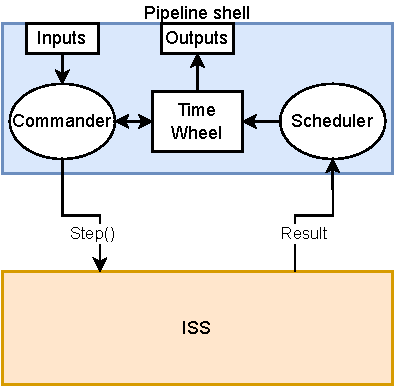
\includegraphics[width=0.5\linewidth]{pictures/time-wheel.pdf}
    \caption{Block diagram of pipeline shell with time wheel.}
    \label{fig:time-wheel}
\end{figure}


\subsection{Comparison}
\label{sec:stageWheelComp}

An important consideration is how the different approaches must be modeled to handle asynchronous events. In the time wheel approach, a single instruction and pipeline stage can have effects stored in multiple cycle slots. Additionally, a single cycle slot can also contain effects from multiple instructions. This can make it difficult to modify single stages or instructions, for instance, to flush a few pipeline stages when taking an interrupt.
On the other hand, the stage-based approach keeps the stage intact, allowing us to halt or flush selected stages more easily.

Another complication for the pipeline simulation is multicycle instructions. Using the CV32E40X core as an example, the longest instruction is the division operation and can last up to 35 cycles \cite{openhw_group_pipeline_2023}. To correctly model this in the time wheel approach, the scheduler needs to know the correct cycle count when inserting the instruction into the time wheel, and the time wheel must be large enough to hold all the cycles. In the stage-based design, this can be modeled by stalling the EX stage for the correct number of cycles, simplifying the design. 

Because the stage-based design follows the flow of the RTL pipeline, stalls can be easily modeled since the preceding pipeline stage can signal if it can be updated, and if not, the following stage must stall. In the time wheel approach, the scheduler must determine beforehand if stalls are necessary and insert these into the time wheel.

In summary, the stage-based approach might be the easiest approach to understand and implement, both for normal execution and for modifications due to asynchronous events. However, the different abstraction levels of the time wheel approach can be beneficial to avoid a simulator that too closely copies the core, implementing the same bugs in both. More work should go into further analyzing both, specifically determining how an asynchronous event can be modeled in both, as well as comparing the complexity details closely.





%\begin{table}[ht]
%\centering
%
%\begin{tabularx}{\textwidth}{|p{30mm}|*{2}{>{\arraybackslash} X |}}
%\hline
%\textbf{Feature}                     & \textbf{Stage-Based Pipeline Simulation}                                  & \textbf{Cycle-Based Time Wheel Simulation}                        \\ \hline
%\textbf{Representation}              & Models pipeline as a series of sequential stages                          & Organizes simulation around clock cycles                          \\ \hline
%\textbf{Intuitiveness}               & Mirrors real-world pipeline architecture, providing easy understanding    & Abstracts away pipeline details, making it less intuitive         \\ \hline
%\textbf{Efficiency}                  & Efficiently models instruction movement through pipeline                  & May require more complex data structures and algorithms           \\ \hline
%\textbf{Stall Simulation}            & Seamlessly simulates stalls                                               & May require additional logic for precise stall handling           \\ \hline
%\textbf{Asynchronous Event Handling} & Simpler to handle as stalls and flushing can be applied to specific stages             & Modifications to a stage, like a stall or flush, may be more complex since stages are represented in multiple cycle slots in the time wheel \\ \hline
%\textbf{Implementation Complexity}   & Generally simpler implementation due to direct representation of pipeline & May require more complex scheduling and state management \\ \hline
%\end{tabularx}
%\end{table}

\section{Pipeline shell and ISS interaction and partitioning}
\label{sec:shell_iss_interaction}

This section will cover the interconnection between the Pipeline shell and the ISS.
As discussed in \cref{sec:spike} and \cref{sec:sail}, a common design in ISS implementations is a step function that executes the three functions: fetch, decode, and execute, where the execute function executes the ALU operations and writes back the results to register files. There are multiple ways of connecting the pipeline shell with the ISS, some of which will be discussed below. We assume the ELF file with instructions is loaded into the ISS for all the implementations.

\subsection{Approach 1}
\label{sec:app1}

One approach is shown in \cref{fig:pipeline-iss-1}. This approach assumes a pipeline simulator with a slot for each stage, and the instructions move from slot to slot through the simulated pipeline, as discussed in \cref{sec:stagebased}. 

From the dependency tree in \cref{fig:dependencyTree}, we see that the content of the IF stage does not directly affect whether an interrupt is allowed to be taken in the CV32E40X core. Additionally, as discussed \cref{sec:cv32Pipeline}, the IF stage is only responsible for updating the PC and fetching the instruction from memory but does not yet know what the instruction contains.

Because of this, we can wait until the ID stage before interacting with the ISS. In the ID stage, we fetch and decode the next instruction and load the decoded instruction and the required register values into the ID slot of the pipeline simulator. Because we have the decoded instruction available, we can use this to calculate any hazards, halts, jumps, etc, in the ID stage. In the EX stage, we can use the decoded instructions to calculate halts, branches, etc. 

Because executing and writeback are combined into one function in the ISS, we do not want to call the execute function from the execute stage to avoid the registers being written to at the wrong cycle. Therefore, we wait until the WB stage before running the execute+write-back function for registers to be updated at the correct time. 

Since we decoded the instruction at the correct cycle, the values read from the register files in the ID stage should be correct in the WB. 

One problem with this solution so far is that forwarding is not considered and will not work properly with a RAW hazard since there will be a 2-cycle delay from registers being read in the ID stage and used and calculated in the WB stage.
Additionally, this solution assumes that no side effects are caused by the EX stage. If this is the case, for example, when communicating with the LSU, we might need to apply these side effects separately when simulating the EX stage.
Waiting to run the execute function to the WB stage will also affect branches, as they are taken in the EX stage. Therefore, additional logic must be integrated into the pipeline shell to take branches at the correct cycle. 

\begin{figure}[ht]
    \centering
    \includegraphics[width=0.5\linewidth]{pictures/pipeline-iss-1.pdf}
    \caption{Pipeline shell and ISS interaction approach 1}
    \label{fig:pipeline-iss-1}
\end{figure}

\subsection{Approach 2}
\label{sec:app2}

The second approach is shown in \cref{fig:pipeline-iss-2}. This approach is similar to the approach in \cref{sec:app2}, but splits up execution and write-back.
This requires modifying the ISS to split up execution and write-back, returning a temporary result to the register file with a separate write-back function at a later stage.

This allows us to fetch and decode in the ID stage and use the decoded instruction in the decode stage to calculate hazards, halts, jumps, etc. In the EX stage, we can call the execute function, execute the operation, cause potential side effects, or potentially branch, and get the temporary result from the execute function. In the WB stage, we can pass the temporary result to the write-back function to update the registers at the correct time.
Since this approach reads from the register file in the ID stage and writes back in WB, we get the same dependencies as the RTL implementation. Therefore, we must implement forwarding, complicating things by moving register values between the different pipeline stages.

\begin{figure}[ht]
    \centering
    \includegraphics[width=0.5\linewidth]{pictures/pipeline-iss-2.pdf}
    \caption{Pipeline shell and ISS interaction approach 2}
    \label{fig:pipeline-iss-2}
\end{figure}

\subsection{Approach 3}
\label{sec:app3}

Another approach is similar to the implementation described in \cref{sec:cycle-accurate} and is shown in \cref{fig:pipeline-iss-3}. Here, the ISS is called once per instruction, executing fetch, decode, and execute before the resulting state changes are passed to the pipeline shell. In the pipeline shell, the results are used to calculate the timing. This approach could be implemented in a stage-based design like \cref{sec:stagebased} and a timing wheel approach like in \cref{sec:timeWheel}.

We chose to keep the ISS intact instead of modifying it to split up the register file from the ISS. Keeping the ISS intact allows us to simplify the simulation by not simulating forwarding. This is because when the ISS operates normally, the registers are updated before executing the next instruction, so we avoid simulating forwarding for all instructions. Instead, we must take care of only the specific conditions where hazards exist and cause stalls. 

Since the ISS immediately writes back to the register file, we do not achieve correct cycle-accurate behavior, as all effects of the instruction would be executed in the IF stage. Additionally, since the effects of the instruction are already executed in the IF stage when situations arise where the pipeline must be flushed, the changes done to the instructions still in the pipeline must be reverted. 

To address these challenges, we could have a copy of the register file and CSR registers in the pipeline shell that gets updated at the correct clock cycles and is used to report the state changes through RVFI out of the reference model.

This approach allows us to execute the whole step function in the ISS without much modification. This is also advantageous as different cores could have different requirements for interacting with the ISS at specific cycles, making this solution better suited to support different processor cores. Since the ISS interaction is standardized to a single function, the pipeline simulation is less constrained to the ISS interface. 

Modifying the ISS to separate the register file can also be a tedious task, as the writeback functionality is often written into each specific instruction function in the ISS. Keeping the ISS intact will make it easier to maintain and keep updated.


\begin{figure}[ht]
    \centering
    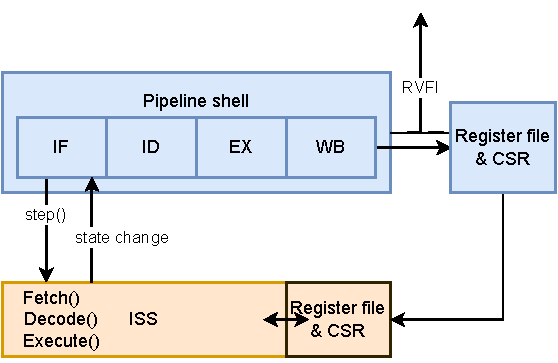
\includegraphics[width=0.5\linewidth]{pictures/pipeline-iss-3.pdf}
    \caption{Pipeline shell and ISS interaction approach 3.}
    \label{fig:pipeline-iss-3}
\end{figure}

\subsection{Comparison of pipeline shell to ISS approaches}
\label{sec:pipeline-iss-comparison}

Considering the three approaches above, each approach has multiple advantages and disadvantages.

Approach 1 and 2 offer a tighter interconnection between the pipeline shell and the ISS, allowing us to utilize more features of the ISS while simulating the pipeline and closer resemblance to the actual RTL implementation. However, this tight coupling requires significant modifications to the ISS, altering the provided interface functions of the ISS and making it more difficult to update the ISS in the future.
By splitting the instruction execution across the different pipeline stages, we alter the fundamental functionality of the ISS, where instead of executing one instruction at a time, it must juggle multiple instructions simultaneously, e.g., fetching one instruction before executing another instruction. This requires a thorough understanding of the ISS to ensure that it still operates as intended and that there are no unobvious interactions between the stages we do not consider.  

Approach 3 circumvents these issues by not splitting up the step execution into multiple stages and instead using the step function often as part of the ISS API, allowing the ISS to fully complete an instruction before moving to the next. This is advantageous because we do not alter the ISS step functionality, and fewer modifications mean the ISS will be easier to keep up to date. Since the interaction between the pipeline shell and the ISS is not dependent on happening in a specific pipeline stage, it also makes approach 3 more adaptable to use with different processor cores. Additionally, by using approach 3, we put fewer constraints on the implementation of the pipeline shell, allowing both the stage-based simulator in \cref{sec:stagebased} and the time wheel simulation \cref{sec:timeWheel} to be used, compared to approach 1 and 2 that only allow the stage-based simulator approach. 
%Since approach 3 is less 

However, approach 3 also requires some modification to the ISS since it requires the pipeline shell to keep track of the state changes. Firstly, the ISS must be modified to report the state changes caused by each instruction when running the step function. Additionally, since we must keep a cycle-accurate version of the processor state outside of the ISS, we need to be able to update the register file and CSR values in the event of a pipeline flush to revert changes already applied to the instructions in the pipeline.

In summary, approach 3 offers the best flexibility and intactness of the ISS and seems like the most suitable approach.

%\subsection{Interrupt passing}
%
%\textbf{TODO}
%
%\subsection{Use register file from ISS or separate register file}
%
%\textbf{TODO}



%\subsection{Approach 4}
%\label{sec:app4}
%
%%Since all instruction essentially executes fully in the IF stage, we can not directly model the pipeline like in \cref{sec:app1} and \cref{sec:app2} above, with the instruction moving from slot to slot. For the next instruction to function properly and have access to the correct data, we can not wait until the WB stage to apply the changes since the next instruction will then calculate with the wrong data. Instead, we can follow the principle from \cite{chiang_efficient_2009}, implementing a time wheel holding all upcoming state changes for each clock cycle, a scheduler handling the implementation details, responsible for filling the time wheel, and a commander that sends commands to the ISS.
%
%When the time wheel reaches the clock cycle with an update event, all effects must be applied. Among other things, this requires updating the GPRs and CSRs used by the ISS.
%
%This requires modifying the ISS so the registers are not updated by the ISS when executing instructions but instead updated by the timing shell at the appropriate clock cycle. 
%
%When an interrupt occurs, the timing wheel must be analyzed to determine if the interrupt can be taken, and the timing wheel must then be updated to reflect the change of PC and flushing of pipeline stages.
%
%\begin{figure}[ht]
%    \centering
%    \includegraphics[width=0.5\linewidth]{pictures/pipeline-iss-4.pdf}
%    \caption{Pipeline shell and ISS interaction approach 4}
%    \label{fig:pipeline-iss-4}
%\end{figure}
%
%
%
%Forwarding control also complicates this design. Since the whole instruction is executed simultaneously, the changes from previous instructions might not be applied yet, as they are applied in WB. 





\section{Choosing base ISS}
\label{sec:choosingISS}

\subsection{Requirements from ISS}
\label{sec:requirements}

To use an ISS as a building block for the reference model, as explained in the previous sections, there are some considerations and requirements to consider that will be listed below. We base the requirements around adhering to approach 3 from \cref{sec:app3}.

\begin{compactenum}[(1)]
    

%\item \textbf{Provide visibility into multiple instructions} \label{req:visibility}
%
%\par To simulate the pipeline, we need to track multiple instructions simultaneously, corresponding to the instructions in the different pipeline stages. This requires that we can "see" the $n$ coming instructions according to the pipeline stages, or allow separation of fetching, decoding, execution, etc into separate cycles. 

\item \textbf{Support stepping through the execution at the Instruction Level} \label{req:step}

\par Since the reference model runs in lock-step with the DUT, we need to be able to step through the instructions at the instruction level, and be able to only run one instruction at a time, before waiting to step into the next instruction.

\item \textbf{Provide processor state after each instruction} \label{req:state}

\par The ISS needs to output the state changes executed after each instruction so that the pipeline shell can apply these changes in a cycle-accurate manner. 
%To be able to use the ISS in verification, we need to access the processor state changes after each instruction to compare with the DUT. This should preferably be in the RVFI format or enough information should be available to convert into an RVFI item.

\item \textbf{Revert the state of the ISS} \label{req:revertState}

\par As discussed in \cref{sec:app3}, if we run the ISS before the pipeline simulation, we need to be able to revert the ISS state to a previous state to simulate pipeline flushing.

%\item \textbf{Support modification of instructions} \label{req:modification}
%
%\par To simulate interrupts in the pipeline, it might be necessary to simulate pipeline flushing and halting. To do this we should be able to modify the instructions in the pipeline e.g. to replace them with empty NOP operations to flush the pipeline or halt execution of an instruction. 

\item \textbf{Enable external injection of interrupts} \label{req:interrupt} 

\par External interrupts and debug requests are inserted into the reference model independently of the ISS. To simulate the interrupts, we must be able to tell the ISS to take an interrupt by jumping to the trap handler's PC and correctly executing the side effects at the correct cycle. 

\item \textbf{Support addition of custom extensions and instructions} \label{req:custom}

\par A large driving force for using RISC-V is the ability to add custom extensions. Therefore, custom instructions and extensions must be easily created and added to the ISS without modifying large parts of the model.

\item \textbf{Ensure maintainability while meeting requirements} \label{req:update}

\par The ISS should be easily maintained and updated while still meeting the requirements. Modifications to the ISS should be kept to a minimum and be done in a way that allows the ISS to be easily updated.

\item \textbf{Actively maintained and thoroughly tested} \label{req:maintained}

\par The ISS should be mature and thoroughly tested. It should be actively maintained and likely to be updated in the future.


\item \textbf{Load the same instructions as the DUT} \label{req:DUTins}

\par The ISS should be able to load the same instructions as the DUT.

%\par As discussed in \cref{sec:shell_iss_interaction}, to be able to model the reference model around an ISS, it is helpful to be able to separate the register file from the rest of the ISS, or be able to have a copy of the register file, and update the register file inside the ISS when necessary.

\end{compactenum}

%\begin{enumerate}[(1)]
%\item Externally inject interrupts to the ISS or modify PC to trap handler 
%\end{enumerate}
%
%The ISS must 
%
%\begin{enumerate}[]
%    \item The execution of the ISS can be modified from the outside to change the instruction, change the program counter, and discard instructions. This should be possible at run-time at every new instruction.
%\end{enumerate}
%sasdfasdfasdf ISS must 
%\begin{enumerate}[resume]
%    \item Should be steppable at the instruction level
%    \item We should be able to "see" multiple instructions. E.g. the 4 instructions in the pipeline
%    \item The ISS should be able to follow the requirements while being easily maintained and kept up to date. E.g. the ISS should not be modified to a point where updating the ISS is not easily done. 
%    \item It should be easy to add custom extensions and instructions to the ISS.
%    \item The ISS should preferably be open-source. 
%    \item The ISS should be actively maintained and thoroughly tested
%    \item The ISS should load instructions in the same format as the DUT. 
%    \item The processor state changes should be available after each instruction
%
%\end{enumerate}

\subsection{ISS comparison}

%\Cref{tab:issComp} shows a comparison between the different Instruction Set Simulators.
%
%\begin{longtable}{|l|p{0.4\textwidth}|p{0.4\textwidth}|}
%\hline
%\textbf{ISS} & \textbf{Pros}                                                                                           & \textbf{Cons}                                                                                                     \\ \hline
%riscvOVPsim  & - Free and open-source                                                                                    & - Very basic                                                                                                       \\ 
%             &                                                                                                           & - Lacking tracing and GDB interface                                                                                \\ 
%             &                                                                                                           & - Dependent on Imperas to add custom extensions                                                                                             \\ \hline
%riscvOVPsimPlus  & - Supports trace and GDB interface                                                                        & - Dependent on Imperas                                                                                             \\
%             &                                                                                                           &                                                                                                                    \\ \hline
%GEM5         & - Recently added support for RISC-V                                                                       & - Intended for architectural exploration and peroframnce simulation                                                \\
%             & - Cycle-accurate simulator                                                                                & - RTL level simulator, might have the same bugs as RTL code                                                        \\
%             & - Features multiple CPU models                                                                            & - An existing model must be modified to match the DUT core                                                         \\
%             &                                                                                                           & - Has no trace output                                                                                              \\
%             &                                                                                                           & - Has limited support for RISC-V extensions                                                                        \\
%             &                                                                                                           & - Must be modified to support lock-step execution                                                                  \\ \hline
%QEMU         & - Full system emulator                                                                                    & - Built to run as fast as possible                                                                                 \\
%             &                                                                                                           & - Uses dynamic binary translation, making it difficult to run a single instruction                                 \\
%             &                                                                                                           &                                                                                                                    \\ \hline
%rv8          &                                                                                                           & - Focus on performance, not accuracy                                                                               \\ \hline
%TinyEMU      & - Small and simple                                                                                        & - Not actively maintained                                                                                          \\
%             & - system emulator                                                                                         &                                                                                                                    \\ \hline
%MARSS-RISCV  & - Cycle-level accurate                                                                                    & - Not actively maintained. Last commit in 2020                                                                     \\
%             & - Simulates both Out-of-order and in-order (6 or 5 stages pipeline) cores                                 & - Has old unfixed bugs                                                                                             \\
%             &                                                                                                           & - Hard to get up to date                                                                                           \\ \hline
%R2VM         & - Simulates a simple 5 stage in-order pipeline                                                            & - Buildt with rust, which is hard to run in conjunction with a SystemVerilig testbench                             \\
%             &                                                                                                           & - Uses dynamic binary translation                                                                                  \\
%             &                                                                                                           & - Focused on performance, not accuracy                                                                             \\
%             &                                                                                                           & - Interrupts are only handled at the end of code blocks                                                            \\
%             &                                                                                                           &                                                                                                                    \\ \hline
%Spike        & - Has been the official RISC-V ISS                                                                        & - Custom instructions must be added in Spike as well as the core                                                   \\
%             & - Thurougly used and tested                                                                               &                                                                                                                    \\
%             & - Supports many extensions                                                                                &                                                                                                                    \\
%             & - Easy to run single instructions                                                                         &                                                                                                                    \\
%             & - Can be split up in modular components. e.g. fetch and debug independently of execution                  &                                                                                                                    \\
%             &                                                                                                           &                                                                                                                    \\ \hline
%sail-riscv   & - The sail-riscv model has been adopted as the formal specification of the RISC-V ISA                     & - The c-emulator consists of a mix of autogenerated code and wrapper code, which can be complicated to work around \\
%             & - Autogenerates a C-emulator from the model                                                               & - The model must be modified to support splitting up the model into separate components like fetch, debug, and execute   \\
%             & - Custom instructions are already specified in sail, so they can automatically be modeled by the emulator &                                                                                                                  \\
%             & - Supports RVFI trace output                                                                              &                                                                                                                  \\ \hline
%                                                                                                         
%\caption{Comparison between different Instruction Set Simulators.}
%\label{tab:issComp}
%\end{longtable}

To find the most appropriate ISS to build the model around, we can apply the requirements from \cref{sec:requirements} to the simulators listed in \cref{back:iss} to see which ISS fulfills all requirements.  

QEMU (\cref{sec:qemu}), rv8 (\cref{sec:rv8}), and R2VM (\cref{sec:R2VM}) all use dynamic binary translation to translate code blocks from RISC-V to the target ISA. This achieves good performance but makes it harder to step through the execution at the instruction level, therefore not meeting \requirement{req:step}. Additionally, interrupts can not be inserted in the middle of a basic block, not meeting \requirement{req:interrupt}. Therefore, we will not consider these further.


RiscvOVPsim (\cref{sec:riscvOVPsim}) is a stable simulator but is closely tied to Imperas. Custom extensions can not be added without buying a license from Imperas, only partially fulfilling \requirement{req:custom}, as we want the solution to be easy to get up and running without acquiring licenses and contacting Imperas. 

%riscvOVPsim - no custom instructions. Has to contact imperas. Not a strict requirement, but an advantage if we can get a fully open source solution. Ease to get up and running without aquiring licences and contacting imperas.


This leaves us with Spike and sail-riscv, which will be compared further below.

\subsection{Spike}
\label{sec:spike_req}

%Spike is popular and widely used, so it is likely to be up to date for a while.
%
%Spike is also used in the verification of other RISC-V cores CVA6 and Ibex 

Looking at the requirements from \cref{sec:requirements}, we will determine which requirements are passed below.

To integrate Spike into the reference model, it is possible to make a copy of the \lstinline{step()} function in \lstinline{execute.cc} to base the model on. This is the same approach as the CVA6 and Ibex spike implementations in \cref{back:cva6} and \cref{back:Ibex}. By using the \lstinline{step()} function, we can make sure we only step one instruction at a time, solving \requirement{req:step}.


%The code below shows a step in the \lstinline{step()} function:
%\begin{lstlisting}[caption={step function in execute.cc from \cite{noauthor_spike_2023}}, label={codef:execute}, language=c]
%for (auto ic_entry = _mmu->access_icache(pc); ; ) {
%    auto fetch = ic_entry->data;
%    pc = execute_insn_fast(this, pc, fetch);
%    ic_entry = ic_entry->next;
%    if (unlikely(ic_entry->tag != pc))
%        break;
%    if (unlikely(instret + 1 == n))
%        break;
%    instret++;
%    state.pc = pc;
%}
%advance_pc();
%\end{lstlisting}
%
%
%One way to implement the reference model around Spike could be using a modified version of the step function as the interface between the reference model and Spike. If we use the sequential pipeline simulation approach from \cref{sec:sequentialPipeline}, we could "fetch" instructions into the pipeline with \lstinline{_mmu->access_icache(pc)}. In Spike, the instructions placed in the \lstinline{icache} are already decoded, so we do not have to disassemble them to calculate hazards, etc. 
%
%The pipeline model could store the \lstinline{insn_fetch_t} fetch types for the different pipeline stages, move these around, and use the \lstinline{execute_insn_fast()} function to execute the instructions. This passes \requirement{req:visibility} by storing the different instructions in a pipeline simulator. If we need to modify an instruction to account for an interrupt or something similar, it could be possible to modify the fetch type to hold another instruction, also solving \requirement{req:modification}.  
%
%Doing it like this should make it fairly easy to stall, flush the pipeline, and modify instructions if needed. We also have control over the PC. 

%To integrate Spike according to approach 3 in \cref{sec:app3}, we want to keep Spike as intact as possible. We can use the \lstinline{step()} function to step Spike one instruction at a time. Approach 3 also requires that the state changes from an instruction is output after every instruction retirement.


%we need a way to output an RVFI item at the end of each instruction retirement. Spike does not explicitly support RVFI, but we can extend Spike to build an RVFI item using the processor state. 


In Spike, the state, including the register file, CSR registers, and PC, is stored in a \lstinline{state_t} struct in the \lstinline{processor_t} class in \lstinline{processor.h}. To fulfill \requirement{req:revertState}, we should be able to revert this state to a previous state. One possibility is for the pipeline shell also to contain a \lstinline{state_t} struct that is updated cycle-accurately from the pipeline shell. The \lstinline{processor_t} could be expanded with a \lstinline{set_state(state_t state)} method to allow the state to be set from the pipeline shell.

To fulfill \requirement{req:state} we need to output the state changes from Spike after every step. One possibility could be to extend Spike with RVFI support. This is currently in development in the CVA6 Spike implementation in \cref{back:cva6}, which we can use as a starting point. Alternatively, we could use the \lstinline{get_state()} method from \lstinline{processor_t} to output the \lstinline{state_t} type from Spike to the pipeline shell.

To fulfill \requirement{req:interrupt}, we need to be able to insert interrupts before any instruction. This can be done similarly to the Ibex Spike cosimulator approach discussed in \cref{back:Ibex}. This expands Spike with different functions like \lstinline{set_nmi()}, \lstinline{set_mip()}, \lstinline{set_debug_req()}, that modify the correct registers and execute a step to make spike take the interrupt.

Spike has support for a large amount of extensions. It is also possible to add custom instructions by adding a new instruction file in \lstinline{riscv/insns/<new_instruction>.h} and adding the opcode and mask to \lstinline{riscv/opcodes.h} \cite{noauthor_spike_2023}. this makes it relatively simple to add custom instructions and passes \requirement{req:custom}.

Since Spike is the official RISC-V ISS developed alongside the RISC-V specification since 2010, it will likely contain few bugs and continue being supported into the future, fulfilling \requirement{req:maintained}.

To fulfill \requirement{req:update}, pulling a new version of Spike should be simple when it receives updates. We should, therefore, leave Spike as intact as possible and do modifications on a layer above Spike. Essential modifications to Spike can be made using git patches, as is done with the Spike tandem verification for the CVA6 core in \cref{back:cva6}. This allows us to store modifications to the spike code as patches, pull changes to Spike, and then apply these patches.

Spike can be loaded with an ELF file, which is also loaded into the DUTs memory module. This fulfills \requirement{req:DUTins}.

From the above, we see that Spike fulfills all the requirements and is a good choice as an ISS to base the reference model.

\subsection{Sail-riscv}
\label{sec:sail_req}

The sail-riscv c-emulator introduced in \cref{sec:sail} consists of a mix of autogenerated c code generated from the sail model and wrapper code that interacts with the generated code. The interface into the autogenerated code is written in \lstinline{riscv_sail.h} and exposes functions to control the simulator, as well as variables exporting the machine state, such as PC, GPR, some CSR registers, and privilege level.

 
The emulator exposes the \lstinline{zstep()} function to step through one instruction, fulfilling \requirement{req:step}. Fetching, decoding, and execution are all done in this function. 

The sail-riscv model also supports RVFI\_DII (Risc-V Formal Interface - Direct Instruction Injection), which implements both RVFI trace output, as well as direct injection of instructions into the simulator through the DII interface, bypassing the PC and instruction memory \cite{joannou_randomized_2023}. Using the RVFI implementation, we can output an RVFI item after each instruction, fulfilling \requirement{req:state}. 


To fulfill \requirement{req:revertState}, we must be able to revert the ISS state to a previous state. Some of the state variables are available in \lstinline{riscv_sail.h}, which we could use to set each of these back to a value stored in the pipeline shell, but only a few of the CSR registers are available here. To be able to revert all the state variables, we must modify the sail model and \lstinline{riscv_sail.h} to output all CSR registers. Additional testing is required to verify that modifying the values output here modifies the model's internal values.


To inject interrupts into the sail model and fulfill \requirement{req:interrupt}, the model must be modified to expose a function that sets the correct CSR registers at the correct time. These registers are not output from the model, but if the modifications described above are done, outputting all the CSR values to \lstinline{riscv_sail.h}, we can insert interrupts by modifying the CSR interrupts like \lstinline{mip}. 



 
%The approach described in \cref{sec:app1} and \cref{sec:app2}, where we hold each instruction in slots in a pipeline simulator, is more difficult in Sail-riscv. This is because we need to split up the fetch/debug and execution parts of the step function. To do this, we need to modify the model so that the decode and execute functions from the step function are available outside the ISS. Since this requires modifications to the Sail code and the generated C code, this can be complicated.

%Therefore, Sail-riscv might work better with approach 3 from \cref{sec:app3}, where the whole step function is called simultaneously, requiring fewer modifications to the Sail model. If we can use this approach, we should also be able to fulfill \requirement{req:modification}, since we can modify the instructions when they are returned from the ISS to the pipeline shell.

%
%The sail-riscv model incorporates multiple "hooks" that can be used to execute code at different points during execution.
%For accessing and transforming the decoded instructions, we can use
%\lstinline{ext_decode(bv)} from \lstinline{riscv_decode_ext.sail}. 
%
%It is also possible to modify the PC with the functions \lstinline{get_arch_pc(), get_next_pc(), set_next_pc(), and tick_pc()}from \lstinline{riscv_pc_access.sail}
%
%There are also the hooks; \lstinline{ext_fetch_hook()}, \lstinline{ext_pre_step_hook()}, \lstinline{ext_post_step_hook()}, and \lstinline{ext_pre_step_hook()} that are executed at different points during the step function. This could be used to insert specific instructions, for example inserting NOP operations to "flush" the pipeline, etc.
%
%The main code execution happens from \lstinline{riscv_sim.c}. Here the model is initialized and an elf file is loaded into the emulator. 


\requirement{req:custom} is a big incentive for using sail-riscv as the ISS in the reference model. Since the sail model has been adopted as the golden RISC-V model, most extensions are modeled in sail, and custom extensions are also implemented in sail. Using sail as the ISS would allow instructions to be defined in only one place, providing a single source of truth and avoiding differing interpretations of the ISS and specification. 


We have seen above that some modifications to the model or interface might be necessary to meet the other requirements. 
To meet \requirement{req:update} we must make sure that the modifications done are minimal. This can be done by making a copy of the \lstinline{riscv_sail.h} outside of the model to extend the interface or use git patches to ensure that new updates can be pulled without modifying the code.


Regarding \requirement{req:maintained}, sail-riscv is also a fairly mature and safe option, especially since the RISC-V Foundation has adopted it as the formal golden model. It is likely to continue being supported and for more bugs to be found as it gains popularity.



To fulfill \requirement{req:DUTins}, we can either load an ELF file into the emulator or use the DII interface to inject instructions directly into the emulator.


%\cite{noauthor_riscv_2023}

%Generating the reference model from the sail model would be optimal for keeping up with changes and easily supporting extensions. As the sail model is the golden risc-v model and custom extensions and instructions are often added to the sail model already, it makes sense to use the sail model as the base ISA. This would allow instructions to only be defined in one place and not modified in both the model and reference model. For this to make sense, the sail model should be held relatively intact so it can be kept up to date with the latest updates.


%. This could allow us to have more control over the instructions to be executed. DII allows direct injection of instructions into the model, which outputs an RVFI trace of the given instruction. The DII bypasses the PC and instruction memory, loading instructions directly into the IF/ID register. Using this method, the reference model would therefore have to handle the instructions instead of loading an elf file into the model. The model would probably also have to decode the instructions outside of sail to know how to handle the instructions. This method would greatly increase the control of when and what instructions are executed, and handling branches would be easier, but there would be some double work e.g. as instructions are already decoded inside sail, but would also be decoded in the reference model. 
%
%The DII\_RVFI interface uses network socket design, so the simulator would have to support sending and receiving instructions and traces through a socket. 
%
%The RVFI\_DII (Risc-V Formal Interface) interface can be used to interface with to the model. This requires:
%\begin{itemize}
%  \item The reference model must keep track of the PC and instructions. This gives us control over the pipeline, and we can easily flush, stall, and modify instructions etc. We can also modify the PC and branch to the interrupt handler etc.
%  \item The DII interface is used to inject instructions directly into the IF/ID register. We could model the pipeline to carry the instructions all the way through the pipeline and send the instruction into the model in the WB stage to execute the side effects of the instruction.
%  \item If we assume the instruction is fed back into the ISS at the WB stage, we need to do some disassembly of the instructions in IF to calculate hazards etc. Two options for this is:
%  \begin{itemize}
%      \item Use a separate disassembler to get rs1, rs2, rd, etc. Here support for custom instructions might need to be added to this disassembler as well. (or maybe not since rs1, rs2, and rd are positioned at the same place for all instructions. )
%      \item Use the decoder from the sail model. This requires some fidling and modification of the model to "extract" the decoder and convert the instructions to the correct format. If we do this, custom extension only need to be defined in the sail model and not in another disassembler as well. 
%  \end{itemize}
%  \item Output the RVFI trace out of the reference model to compare with DUT. If we use the RVFI\_DII interface, it should be relatively simple.
%\end{itemize}
%
%
%Another alternative that is a bit more hacky would be to to use the rvfi functions defined in \lstinline{riscv_sail.h} to avoid using the socket. This exposes functions like \lstinline{zrvfi_get_ins()}, \lstinline{zrvfi_set_instr_packet()}, and \lstinline{zrvfi_halt_exec_packet()}. This could allow us to use the same method as with the socket where the reference model controls the instructions and PC. 
%
%It might also be possible to become more tightly coupled with the emulator and have the model load the elf file, and use the functions above to extract information from the instructions and model the pipeline around this. This could get quite messy.
%
%The CORE-V verification also utilizes RVFI tracing for step-and-compare, possibly making the integration with the rest of the verification environment easier.



%The sail model without modification has no obvious method to be able to use the sail model to disassemble the instruction without executing the instruction. Some form of disassembly is required to calculate hazards etc. in the pipeline. In the RISC-V ISA, the source and destination registers are in the same position for all instructions, so basic decoding of registers is possibly not too complicated. \cite{waterman_risc-v_nodate}


%\subsubsection{sail hooks}
%
%The sail-riscv model incorporates multiple hooks that can be used to execute code at different points during execution.
%For accessing and transforming the decoded instructions, we can use
%\lstinline{ext_decode(bv)} from \lstinline{riscv_decode_ext.sail}. 
%
%It is also possible to modify the PC with the functions \lstinline{get_arch_pc(), get_next_pc(), set_next_pc(), and tick_pc()}from \lstinline{riscv_pc_access.sail}
%
%There are also the hooks; \lstinline{ext_fetch_hook()}, \lstinline{ext_pre_step_hook()}, \lstinline{ext_post_step_hook()}, and \lstinline{ext_pre_step_hook()} that are executed at different points during the step function. This could be used to insert specific instructions, for example inserting NOP operations to "flush" the pipeline, etc.



\subsection{Spike vs. Sail}

\Cref{tab:spikevsail} shows the advantages and disadvantages of using Spike and Sail-riscv as the ISS the model is built around

\begin{table}[!htb]
\centering
%\setlist[itemize]{font= \color{DeepSkyBlue}, wide, leftmargin=*, noitemsep, after=\vspace*{-\topsep}}
%\setlength{\extrarowheight}{3pt}
%\setlength{\tabcolsep}{3pt}
\caption{Summary of advantages and disadvantages of Spike and Sail-riscv}
\label{tab:spikevsail}
%\begin{tabularx}{\textwidth}{|p{15mm}|*{2}{>{\compress\RaggedRight\arraybackslash} X |}}
\begin{tabularx}{\textwidth}{|p{15mm}|*{2}{>{\arraybackslash} X |}}
\hline
ISS & Advantages & Disadvantages \\
\hline
Spike
& \begin{itemize}
\item Widely used and tested 
\item Extensive support for many extensions 
\item The C++ code is easy to modify and modularize
\item Already integrated into core-v-verif for verification of the CVA6 core
\end{itemize}
& \begin{itemize}
\item Custom instructions must be added separately 
\item Model must be modified to output RVFI trace items at instruction retirement
\item Must be modified to inject interrupts into the model
\end{itemize} \\
\hline
Sail-riscv
& \begin{itemize}
\item Adapted as the official RISC-V specification 
\item Supports RVFI trace output
\item Extensions already modeled in sail, can be automatically added to the model
\end{itemize}
& \begin{itemize}
\item The mix of handwritten and autogenerated sail and C code is complicated to work around 
\item Modifications are necessary to separate fetch/debug and execute functions
\item Must be modified to inject interrupts into the model
\item Not as much used for verification as Spike
\end{itemize} \\
\hline
\end{tabularx}
\end{table}

From \cref{sec:spike_req} and \cref{sec:sail_req}, we see that Spike and Sail-riscv both are viable options to use as the Instruction Set Simulator that the pipeline shell is built around. Both Spike and Sail-riscv can be modeled to fulfill all the requirements in \cref{sec:requirements}, but Spike requires fewer modifications to be able to meet them. There are also some other differences between them, as shown in \cref{tab:spikevsail}. Spike is the most used ISS and has been around since the start of RISC-V. It is a golden model for the RISC-V ISA and many cores. This makes Spike an attractive choice as most bugs are removed, and it has been thoroughly tested and trusted. 

As Spike is fully written in C++, code modifications are easier than Sails' mix of handwritten C code and C code autogenerated sail model. 

Fulfilling \requirement{req:revertState} is easier in Spike than in Sail if we keep a copy of \lstinline{state_t} struct in the pipeline shell and revert the ISS state by using this copy of the state. In comparison, in Sail, we would have to modify the model to export all CSR variables and individually set all of these back to revert the state.

Sail-riscv already has RVFI support, allowing us to output the state changes during each instruction retirement and use this further to output the changes from the reference model to compare the reference model and DUT. For Spike, this RVFI support must be added directly to Spike or the pipeline shell to compare the reference model to the DUT. 
%Specifically considering the separation of fetch/debug and execute discussed in \textbf{LINK}, this is advantageous in Spike. In Spike, we can model the interface around the step function and easily separate the fetch/debug and execute stages, while in Sail, these are all embedded into the same step function accessible from outside the model, requiring modifications to the model to separate these, or modifications to how the ISS is integrated with the pipeline shell.

Spike has been used to verify multiple cores, including the CVA6 core from OpenHW Group. CVA6 uses the same verification environment as the CV32E40X core we use as an example core. Recent efforts have been made to include Spike in the "core-v-verif" verification environment, and it is therefore also available to use with the CV32E40X. The CVA6 Spike implementation has already modified the Spike code to make it suitable for verification. Some of these changes can be useful for us, for example RVFI support is in development. 

%We will also need to modify the Spike code if it is used in the reference model. One disadvantage of using the same Spike implementation as the CVA6 core is that the modifications required by the Reference Model might differ from those required by CVA6, leading to chaos if improperly organized.


Regarding interrupts and debug requests, both Spike and Sail-riscv require modifications to the code to add functions for inserting interrupts into the simulator. This has previously been done for the Ibex co-simulator for Spike, but for Sail-riscv, this needs to be investigated further. 

Sail-riscv is more advantageous than Spike in regards to custom extensions. Since Sail has been adopted as the official specification, most custom extensions are already modeled in Sail. These custom extensions can be added to the model and automatically added to the reference model.  Doing this means that the sail specification can serve as a single source of truth in the reference model, the specification, and possibly in formal models. In comparison, in Spike, we need to separately add all the functionality of a custom extension to the Spike simulator, which can lead to bugs in the Spike modeling. On the other hand, if there is a bug in the Sail specification, this can be present both in the RTL code and the reference model and can be hard to find. 


The discussion above shows that both Spike and Sail-riscv seem to be suitable options, as they can be modified to meet all requirements. However, Spike will be easier to modify because of its C++ code, compared to the mix of c and autogenerated Sail code in Sail-riscv. Because of this, and other the reasons listed above, Spike might get us up and running faster, allowing more work to be done on the more complicated implementation of the pipeline shell. If possible, the interface between the reference model and ISS should be relatively generic, so switching from Spike to Sail in the future should be possible if desired.

%that Spike seems more suitable but is not necessarily the only possible choice. Both Spike and Sail-riscv can be modified to meet all requirements,




%\subsection{Core configuration}
%
%The reference model should be easily configurable.
%
%To achieve this....